\chapter{Systemmodell}
Die Rechteverwaltung basiert auf \glspl{Gruppe}. Jede Gruppe hat verschiedene Berechtigungen. Im Folgenden wird zwischen \gls{Reviewer}n, \glspl{Nutzer}n und \glspl{Admin} unterschieden.
Jede höher liegende Gruppe kann alle Funktionen der darunter liegenden Gruppe nutzen.
%Es wird bei der Ansicht der Workflows nicht zwischen \gls{Nutzer}n, \gls{Reviewer}n und \glspl{Admin} unterschieden. 

\gls{Reviewer} können sich anmelden, abgeschlossene Workflows einsehen und aktuell laufende \gls{Workflow}en einsehen.

\gls{Nutzer} können /M10/, /M20/, /M30/, /M40/, /M50/, /M60/, /M70/ und alle Funktionalitäten, die \gls{Reviewer} nutzen können, nutzen.

\gls{Admin} Nutzer können die Funktionen /M80/, /M90/, /M100/ und alle Funktionen, die \gls{Nutzer} und \gls{Reviewer} ausführen können, ausführen.

%Nochmal am Ende anschauen und links fixen

\begin{figure}[ht]
    \centering
    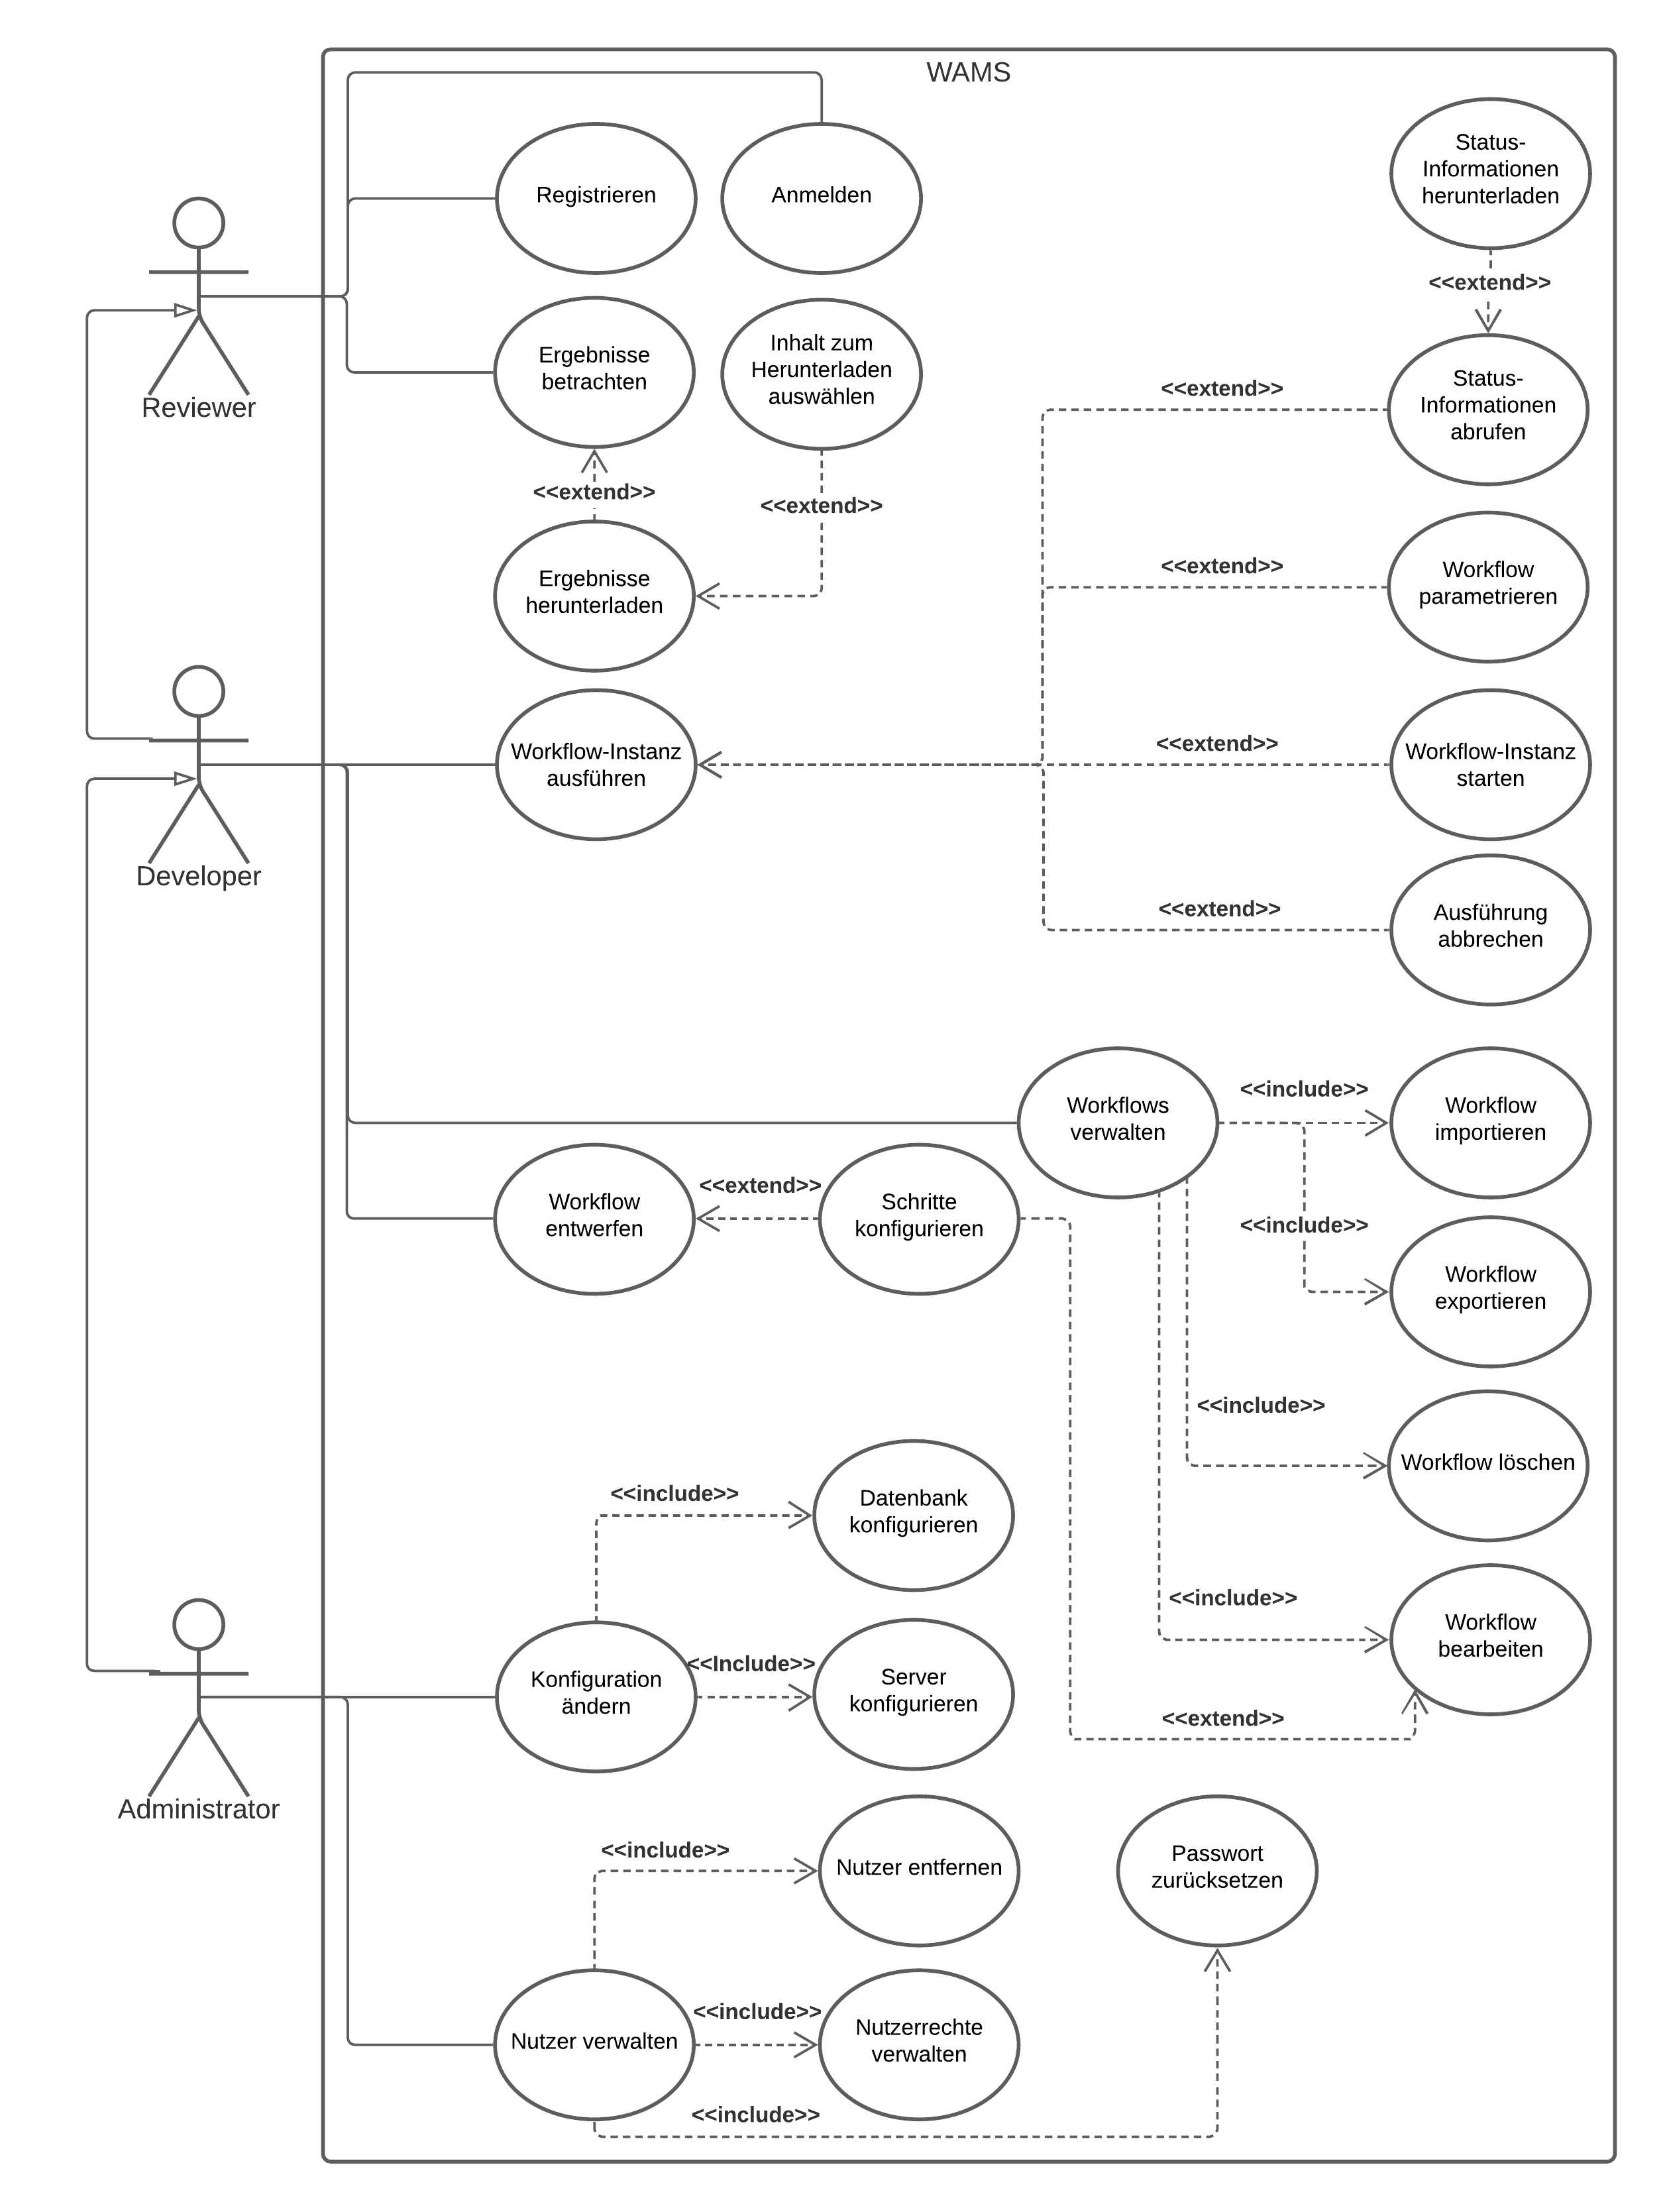
\includegraphics[width = \textwidth]{Grafiken/Diagramme/Anwendungsfalldiagramm.png}
    \caption{Anwendungsfälle und Verteilung der Rechte und nutzbarer Funktionen}
    \label{fig:Anwfalldiag}
\end{figure}